\documentclass[11pt]{article}
\usepackage[utf8]{inputenc}
\usepackage[french]{babel}
\usepackage{graphicx}
\usepackage[T1]{fontenc}
%\usepackage{amss}
\usepackage{amsmath}
\usepackage{amsfonts}
\usepackage{amssymb}

\newcommand\comment{}
 
\def\N{\mathbb N}
\def\R{\mathbb R}
\def\Q{\mathbb Q}
\def\Z{\mathbb Z}
\begin{document}
\title{EXAMEN D'ALGORITHMIQUE, I31A}
\date{}%{12-12-2013}
%\maketitle
{\bf\large EXAMEN D'ALGORITHMIQUE, I31A, 12-12-2013, L2} 

\medskip

{\it Tous vos documents sont autorisés, mais pas la copie de votre voisin.
N'écrivez aucun programme.
Ecrivez lisiblement.
Répondez aux questions dans l'ordre, en indiquant le numéro de chaque question.
}

\newcommand\q[1]{\medskip \noindent {\bf #1.}}
\medskip 

\q{1}  {D\'eroulez l'algorithme d'Euclide pour calculer le PGCD de 132 et 102}.

\medskip
pgcd(132, 102)= pgcd( 102, 30) = pgcd( 30, 12)=pgcd( 12, 6)= pgcd( 6, 0)= 6

\q{2} {D\'eroulez l'algorithme d'Euclide \'etendu (ou Bézout) pour $a=132$ et $b=102$ en remplissant un tableau comme ci-dessous. {\it Dans la dernière ligne, $b$ est nul et $a$ est le PGCD cherché}.
L'algorithme vu en cours calcule $g$ le PGCD de $a$ et $b$, ainsi que $u$ et $v$. $u$ et $v$ sont tels que $au+bv=g=PGCD(a,b)$; on note $r=a \mod b$, et $q=\lfloor \frac{a}{b}\rfloor$
le quotient de $a$ par $b$.   Il n'y a qu'une seule réponse correcte.
\medskip


{\large
$$
\begin{array}{|c|c|c|c|c|c|c|}
\hline
a\quad & b \quad& r \quad& q \quad& g \quad& u \quad& v \quad\\
\hline
132 & 102 & 30 & 1 & 6 & 7 & -9 \\
102 & 30  & 12 & 3 & 6 & -2 & 7 \\
30 &  12  & 6  & 2 & 6 & 1 & -2 \\
12 &  6   & 0  & 2 & 6 & 0 & 1 \\
6 &  0   & *  & * &  6 & 1 & 0 \\
\hline
\end{array}$$
}
Donc $(a,b)=(132,102) \Rightarrow (g,u,v)=(6,7,-9)$.

\q{3} (suite) De la solution $(u, v)$ du problème précédent, déduisez d'autres solutions pour $u$ et $v$.
Donnez la formule qui donne toutes les autres solutions.

\medskip

Si $(u,v)$ est tel que $au+bv=pgcd(a,b)$, alors $(u+b,v-a)$ aussi, et
$(u+tb, v-ta)=(7+102\times t, -9 - 132 t)$ pour $t\in \Z$. Donc: $(109, -141),
(-95, 123)$, etc 
~

\q{4} (suite) Quand vous remplissez les cases des colonnes $u$ et $v$, en fonction du contenu de la ligne d'après ou d'avant, quelles formules utilisez vous~?
Réponse suggérée~: soient $(g', u', v')$ le contenu de la ligne en dessous (ou au dessus?).
Alors $(g,u,v)=(g',?,?)$. La preuve n'est pas demandée.


\medskip

Soient $(g', u', v')$ le contenu de la ligne en dessous; alors $(g, u, v)=(g', v', u'-q\times v')$

\q{5} Citez deux problèmes indécidables en informatique.

\medskip

Le problème de l'arrêt (d'un programme ou d'une machine de Turing); l'égalité de deux nombres réels; l'égalité de deux fonctions.


\q{6} Quand un problème, bien que décidable, est-il jugé difficile en informatique ?


\medskip

Quand aucun algorithme en temps polynomial n'est connu.

\q{7} Citez un problème décidable mais difficile en  informatique.

\medskip

Résoudre un problème SAT. Trouver un chemin ou un circuit hamiltonien (passant par tous les sommets dans un graphe). Trouver une clique max ou un stable max. Factoriser un très grand entier.


\q{8} La phrase suivante est-elle vraie ou fausse~: Si un problème est NP, alors il est difficile de vérifier une de ses solutions. 

\medskip
Elle est fausse.

\q{9} {Citez les noms de 3 algorithmes {\it  optimaux}  de tri, utilisant des comparaisons. Quel est l'ordre de grandeur du nombre de comparaisons, pour trier $n$ éléments~?}
  
\medskip
Le tri par fusion (mergesort), le tri par tas (heapsort), le tri rapide (quicksort) probablement rapide, le tri par insertion dans un arbre équilibré.


\q{10} {Citez le nom d'un algorithme efficace de tri d'entiers, qui ne compare pas les entiers entre eux.}
  
\medskip

Le "radix sort", ou tri par base.
  

\q{11} {Déroulez l'algorithme précédent sur cet ensemble: 312, 323, 313, 113, 123, 213, 111, 131, 221. Vous n'utiliserez que trois tiroirs.}
  
\medskip

La première étape range les nombres dans 3 tiroirs 1, 2, 3 selon le chiffre des unités: 

 1: 111, 131, 221.

 2: 312

 3: 323, 313, 113, 123, 213.

L'ordre est: 111, 131, 221, 312,  323, 313, 113, 123, 213.  
La deuxième étape  range les nombres dans 3 tiroirs  selon le chiffre des dizaines:

 1: 111,  312,  313, 113,  213

 2:  221, 323, 123

 3: 131.

L'ordre est:  111,  312,  313, 113,  213, 221, 323, 123, 131.
La troisième et dernière étape  range les nombres  selon le chiffre des centaines:

 1:  111, 113,  123, 131

 2: 213, 221

 3: 312, 313, 323.

L'ordre est: 111, 113,  123, 131, 213, 221, 312, 313, 323. Les éléments sont bien ordonnés de façon croissante.


\q{12} Que fait l'algorithme de Dijkstra (celui vu en cours)~?
\medskip


Il calcule les chemins les plus courts d'un sommet source à tous les autres sommets d'un graphe. Le graphe est orienté. Les arcs ne portent que des longuers non négatives.



\q{13} {$A$ est une matrice de $l_A$ lignes et $c_A$ colonnes; $B$ est une matrice
de $l_B$ lignes et $c_B$ colonnes. Quand le produit $A\times  B$ est-il possible ?
Quelle est la taille de la matrice $C=A\times B$, quand ce produit est possible? 
Donnez la formule pour $C_{l,c}$ ($C_{l,c}$ est l'élément à la ligne 
$l$ et à la colonne $c$ de 
$C=A\times B$); vous supposerez que la première ligne (ou colonne) a le numéro 1.
Combien de multiplications (entre éléments des matrices) sont effectuées au total, 
pour calculer $C$~?


\medskip

Comme $C_{l, c}$ est le produit scalaire de la ligne $l$ de $A$ par la colonne $c$ de $B$, il faut que 
il faut que $c_A=l_B$. La matrice $C=A\times B$ a $l_A$ lignes et $c_B$ colonnes.
$$C_{l,c}=\sum_{k=1}^{c_A} A_{l,k} \times B_{k, c}$$
Il faut $l_A\times c_A \times c_B= l_A\times l_B \times c_B$ multiplications entre nombres pour calculer $C$.

\q{14} {Donnez les {\it formules} n\'ecessaires pour le calcul r\'ecursif 
et {\it rapide} de $a^n$ ($a$ est une matrice carrée, à valeurs enti\`eres;  
vous noterez la matrice identité $I$). N'oubliez pas le ou les cas terminaux. 
Il est inutile de redonner les formules pour le produit de 2 matrices. 
Quel est l'ordre de grandeur du 
nombre de multiplications  matricielles effectuées pour calculer $a^n$~?}  


\medskip

$a^0=I,\quad a^1= a,\quad a^{2k}=(a\times a)^k,\quad a^{2k+1}= a\times a^{2k}$
On suppose que l'exposant est non négatif et que $a$ est carrée.
La seconde règle est facultative. 
Tous les deux appels récursifs au plus, l'exposant est divisé par 2, donc
il y a au plus $2 \log_2 n = O(\log n)$ appels récursifs et multiplications de matrices.  

\q{15} {Dans la question précédente, pourquoi les formules: $a^0=I, a^1=a, a^{k+1}=a \times a^k$ ne sont elles pas satisfaisantes~?}

\medskip

Cet algorithme utilise $O(n)$ produits matriciels au lieu de $O(\log n)$.

\q{16} {Quel est le nom de la méthode utilisée pour résoudre "le problème des reines" et "le compte est bon"~?}

\medskip

"backtrack" (recherche arborescente avec retour arrière).

\q{17} Un arbre binaire a $F$ feuilles; $F\ge 1$. 
Tous ses noeuds intérieurs (non feuilles) ont exactement deux fils.
L'arbre n'est pas forcément équilibré. Est-il possible de dire combien 
il a de noeuds intérieurs, ou bien le nombre de noeuds intérieurs peut-il varier~?
Donnez le nombre de  noeuds intérieurs, si ce nombre est fixé par $F$. Prouvez votre réponse.
{\it Rédigez votre preuve  avec soin}.

\medskip


L'arbre a $I=F-1$ noeuds internes. Preuve: chaque feuille représente un joueur (de tennis par exemple). Chaque noeud représente une rencontre qui oppose exactement  deux joueurs et est étiqueté avec le gagnant. La racine de l'arbre est étiqueté avec le gagnant du tournoi. Comme chaque rencontre élimine un joueur (le perdant),
et que $F-1$ joueurs doivent être éliminés,
il faut $I=F-1$ rencontres (ou noeuds internes). Donc l'arbre a $I=F-1$ noeuds internes.
CQFD.

\q{18} La suite $T$ est définie par: $T_0=T_1=1, \quad T_{n+2}= T_{n+1}+ T_{n} + 1 $.
En vous inspirant du cas de la suite de Fibonacci, donnez une formule matricielle
exprimant le vecteur  colonne~:  
$(T_{n+2}, T_{n+1}, 1)$ en fonction d'une matrice, que vous préciserez, et du vecteur
colonne $(T_1, T_0, 1)$. Donnez ensuite le principe d'une méthode
rapide pour calculer $T_n$. Quelle est sa complexité, en fonction de $n$~?

\medskip

$$\left(\begin{array}{c}
T_{n+2} \\
 T_{n+1}\\
1 \\
\end{array}\right)= \left(\begin{array}{ccc}
1 & 1 & 1 \\
1 & 0 & 0 \\
0 & 0 & 1 
\end{array}\right)\left(\begin{array}{c}
T_{n+1}\\
T_n \\
1\\
\end{array}\right)= \left(\begin{array}{ccc}
1 & 1 & 1 \\
1 & 0 & 0 \\
0 & 0 & 1 
\end{array}\right)^{n+1}\left(\begin{array}{c}
T_{1}\\
T_0 \\
1\\
\end{array}\right)$$

Donc la puissance rapide de cette matrice permet de calculer $T_k$ en $O(\log k)$ produits matriciels. 

\q{19} L'équation~: $ax^2+bx+c=0$ est
résolue par l'itération de Newton (ou de Newton-Raphson); $a\neq 0, b, c \in \R^3$ ont des valeurs données.
Donnez la formule pour l'itération de Newton; $N(x)=?$. 
Il est demandé de remplacer $f(x)=ax^2+bx+c$ et $f'(x)$ par leurs valeurs.

\medskip
$$ N(x)=x - \frac{f(x)}{f'(x)} = x - \frac{ax^2+bx+c}{2ax+b}= \frac{ax^2-c}{2ax+b}$$


\q{20} (suite) Donnez des valeurs numériques de $a, b, c$ et deux valeurs distinctes $x_0, x_1$ pour lesquelles $x_1=N(x_0)$
et $x_0=N(x_1)$. Autrement dit, l'algorithme boucle.  Choisissez des valeurs simples. Illustrez votre exemple par un dessin.

\begin{center}
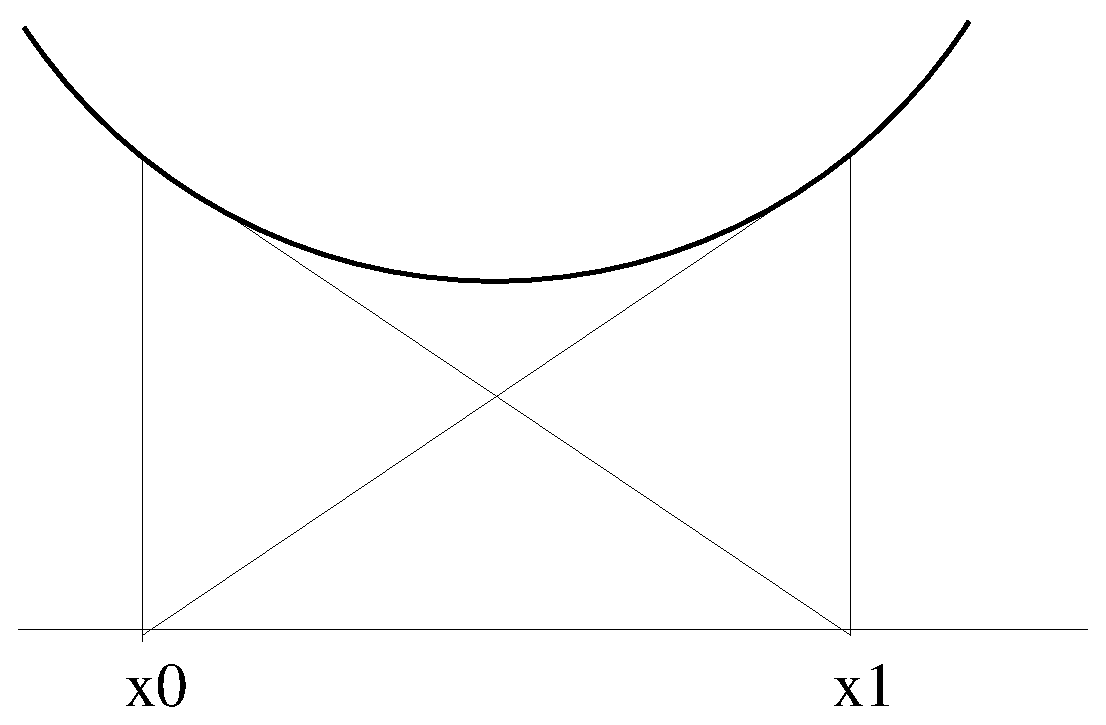
\includegraphics[width=0.5\linewidth]{bouclenewton.eps}
\end{center}
Choisir $f$ paire simplifie les calculs, par exemple $f(x)=x^2+c$, avec $c>0$.
$N(x)= \frac{x^2-c}{2x}$. Prenons $x_1=-x_0$. Alors 
$N(x_0)=x_1=-x_0\Rightarrow 3x_0^ 2=c\Rightarrow x_0= \pm \sqrt{c/3}$.
Pour $c=1$, $(x_0, x_1)= ( \sqrt{3}/3, -\sqrt{3}/3)$ est une boucle.

\q{21}
Votre boucle est attractive ssi $|N'(x_0)\times N'(x_1)| < 1$; l'est elle~?


\medskip

La dérivée de $N$ est $N'(x)= \frac{x^2+c}{2x^2}$.
Donc $|N'(x_0)N'(x_1)|=4$, pour tout $c> 0$. Cette boucle est répulsive: elle ne résistera pas aux imprécisions numériques.
\end{document}
